\section{Технологическая часть}

В данном разделе будет обоснован выбор средств программной реализации предлагаемого метода: выбраны платформа, язык программирования, среда разработки и сборки ПО, используемые расширения, описан формат входных и выходных данных. 
Разработано программное обеспечение, реализующее представленный метод.
Приведен пример работы программы, выполнено тестирование, а также описан способ обращения к программе.

\subsection{Выбор средств разработки}

%\subsubsection{Выбор платформы}
По результатам анализа только исследуемые методы отображения интерфейса нативной мобильной разработки не обладают функцией горячей перезагрузки. 
В связи с чем в качестве платформы разработки для реализации предлагаемого метода выбрана операционная система iOS.

%\subsubsection{Выбор языка программирования}
Выбран язык Swift \cite{swift}, поскольку он является основным используемым в нативной разработке iOS.

%\subsubsection{Выбор среды разработки и сборка программного обеспечения}
Среда разработки~---~XCode \cite{xcode}, поскольку является интегрированной средой разработки программного обеспечения для платформ macOS, iOS, разработанной корпорацией Apple, а также предоставляет возможность запуска разрабатываемого программного обеспечения на симуляторах устройств \cite{simulator}. 
Используется версия XCode 15.3, являющаяся актуальной на момент написания дипломной работы.
Запуск разрабатываемого программного обеспечения происходит на симуляторе устройства iPhone 15 Pro Max, версия iOS~---~17.4 (также является актуальной на момент написания дипломной работы).

%\subsubsection{Используемые расширения}
Для создания представлений используется библиотека UIKit, содержащая полный набор базовых UI--элементов, а также механизмы размещения их на экране. 

% \subsection{Формат входных и выходных данных}
Входные данные для разрабатываемого метода:

\begin{itemize}[label=---]
	\item пользовательский интерфейс;
	\item событие, инициализирующее изменения интерфейса;
	\item XML--файл, организованный специальным образом.
\end{itemize}

Выходные данные для разрабатываемого метода:

\begin{itemize}[label=---]
	\item пользовательский интерфейс, измененный во время выполнения программы.
\end{itemize}

\subsection{Способ обращения к программе}

Разработанная реализация метода представляет собой класс.
Для использования методов класса необходимо разместить файлы с кодом разработанного метода рядом с файлами программы. 
Для корректной работы приложения необходимо, чтобы каждый UIViewController, интерфейс которого будет реализован с помощью разработанного метода, был унаследован от класса, описанного в листинге \ref{code:Controller.swift}. 

\begin{code}
	\captionof{listing}{Класс, от которого наследуется UIViewController}
	\label{code:Controller.swift}
	\inputminted
	[
	frame=single,
	framerule=0.5pt,
	framesep=10pt,
	fontsize=\small,
	tabsize=4,
	linenos,
	numbersep=5pt,
	xleftmargin=10pt,
	]
	{text}
	{code/Controller.swift}
\end{code}

Для обновления интерфейса необходимо вызвать метод reload в методе жизненного цикла ViewDidLoad.

Также необходимо, чтобы UIViewController был внесен в список наблюдаемых объектов. Для этого необходимо добавить в метод жизненного цикла ViewDidLoad строку, представленную в листинге \ref{code:observer.swift}.

\begin{code}
	\captionof{listing}{Внесение UIViewController в список наблюдаемых объектов}
	\label{code:observer.swift}
	\inputminted
	[
	frame=single,
	framerule=0.5pt,
	framesep=10pt,
	fontsize=\small,
	tabsize=4,
	linenos,
	numbersep=5pt,
	xleftmargin=10pt,
	]
	{text}
	{code/observer.swift}
\end{code}

Далее часть интерфейса или полностью весь интерфейс может быть спроектирован путем создания разметки XML--файла, связанного с UIViewController.

\subsubsection{Пример работы}

В качестве примера работы программного обеспечения был спроектирован интерфейс, содержащий фоновое представление белого цвета, на котором по центру располагается UILabel с текстом <<Привет!>>. 
Скриншот представлен на рисунке \ref{fig:example-before}.
Данному интерфейсу соответствует разметка XML--файла, представленная в листинге \ref{code:example-before.xml}.
\clearpage
\begin{figure}[!htb]
	\centering
	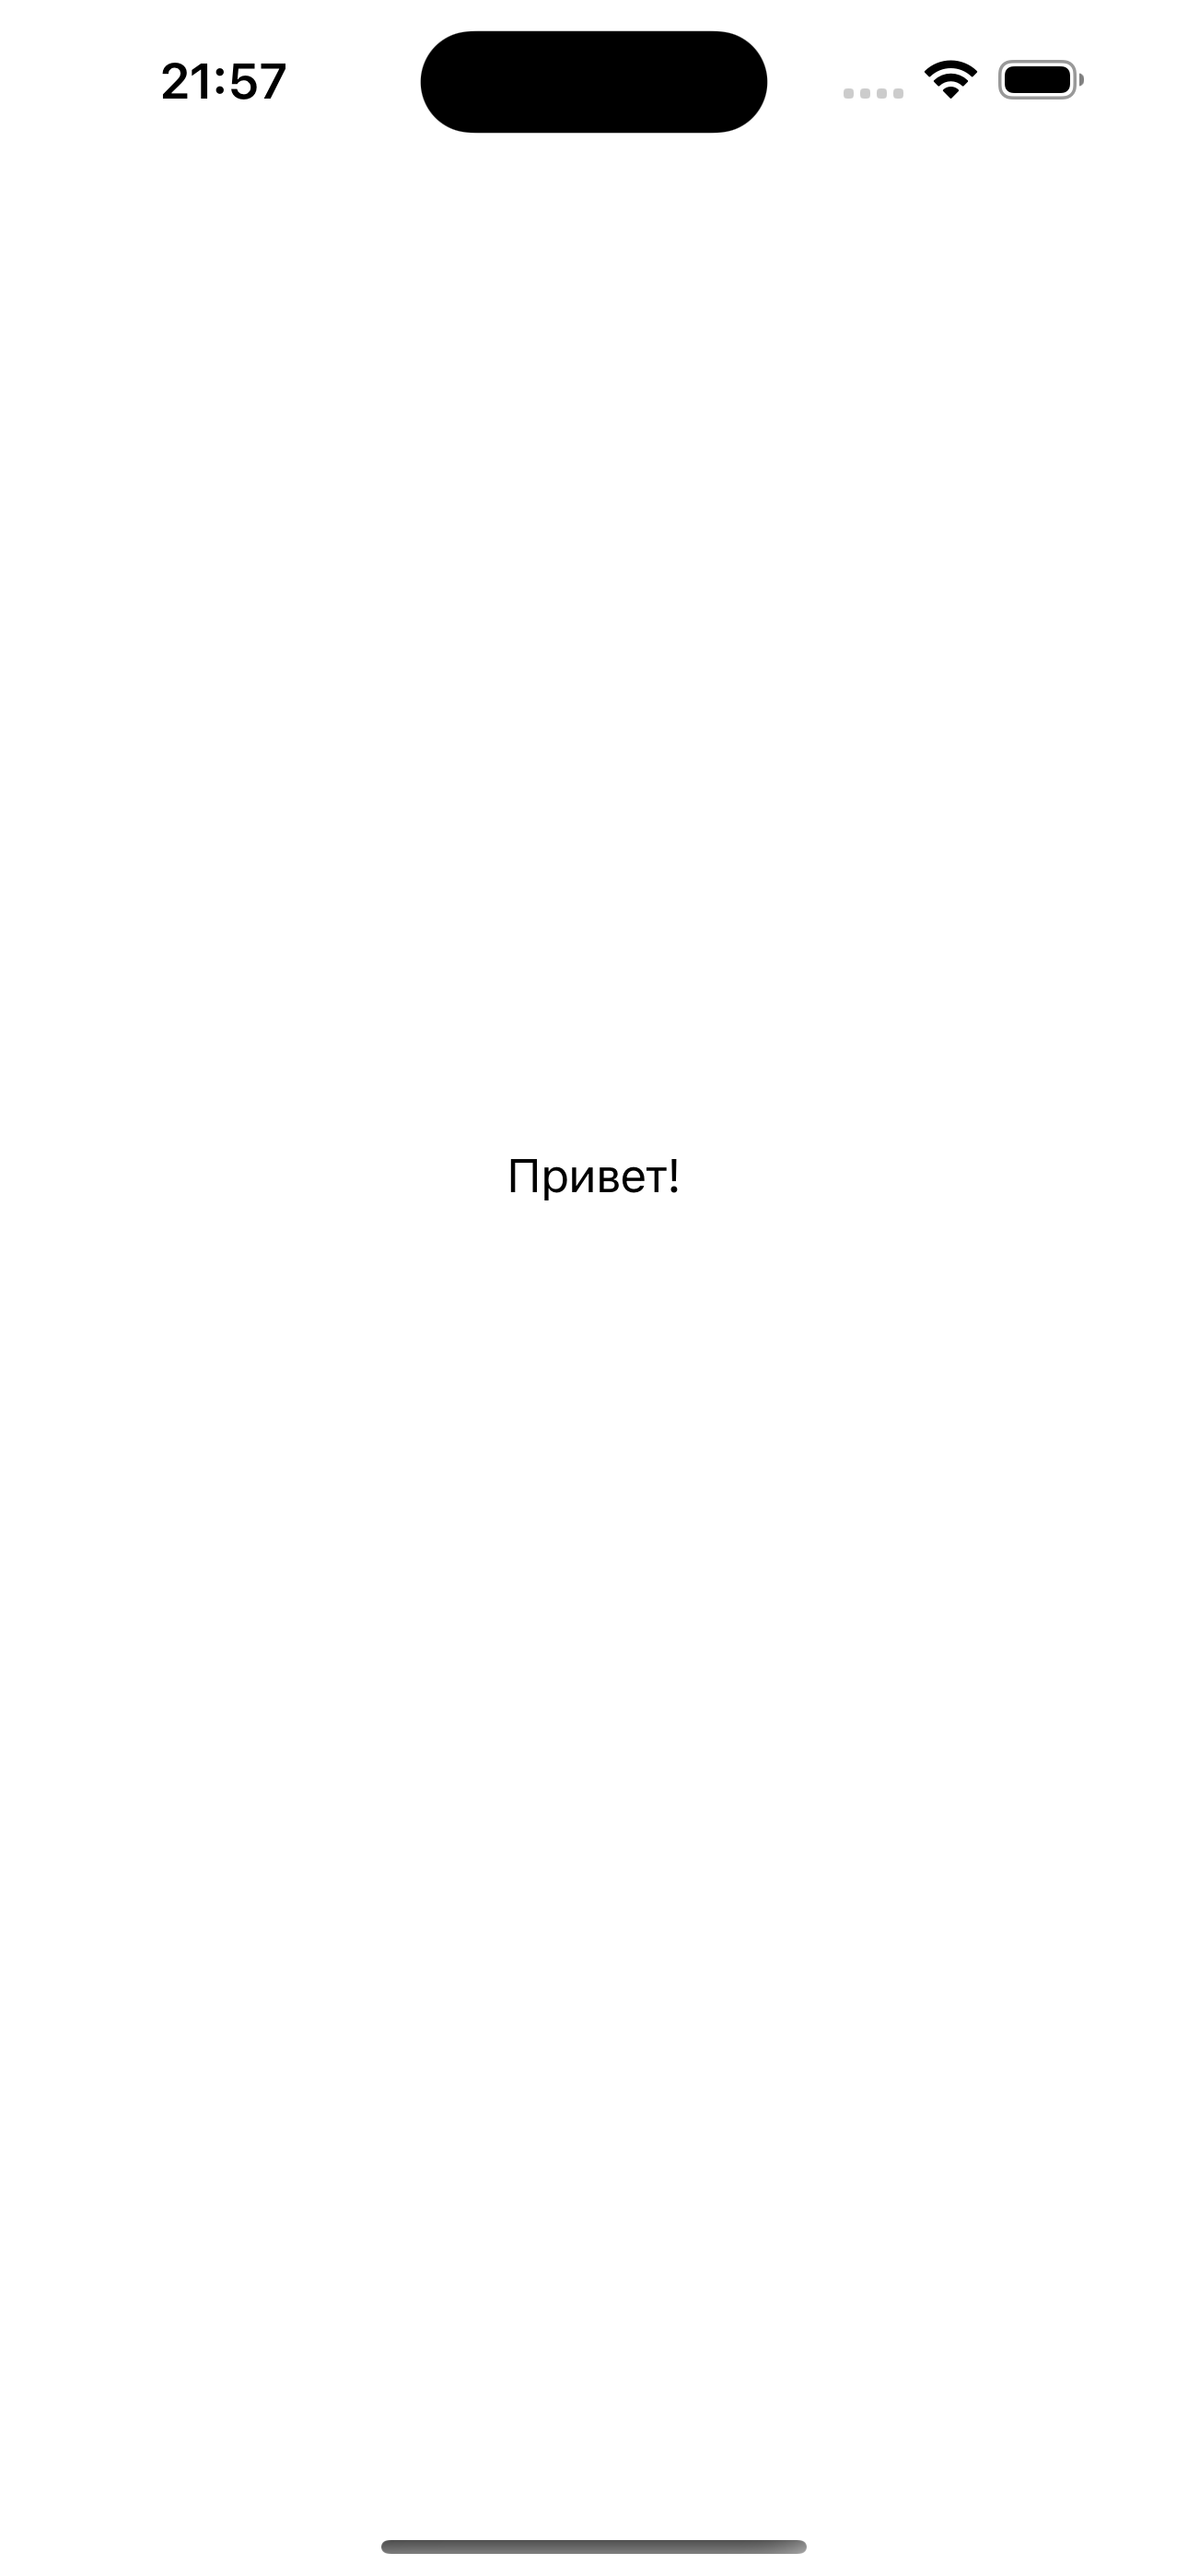
\includegraphics[scale=0.13]{img/example-before.png}
	\caption{Интерфейс до внесения изменений}
	\label{fig:example-before}
\end{figure}

\begin{code}
	\captionof{listing}{Разметка XML--файла до внесения изменений}
	\label{code:example-before.xml}
	\inputminted
	[
	frame=single,
	framerule=0.5pt,
	framesep=10pt,
	fontsize=\small,
	tabsize=4,
	linenos,
	numbersep=5pt,
	xleftmargin=10pt,
	]
	{text}
	{code/example-before.xml}
\end{code}


Во время работы приложения в XML--файл вносятся изменения: на фоновое представление под UILabel добавляется UIView красного цвета, содержащая UILabel с текстом <<Hello!>>. Соответствующая разметка XML--файла представлена в листинге \ref{code:example-after.xml}. 

По нажатию на сочетание клавиш CMD + t ноутбука, на котором запущено программное обеспечение, происходит обновление интерфейса. 
Обновленная версия представлена на рисунке \ref{fig:example-after}.

\begin{figure}[h]
	\centering
	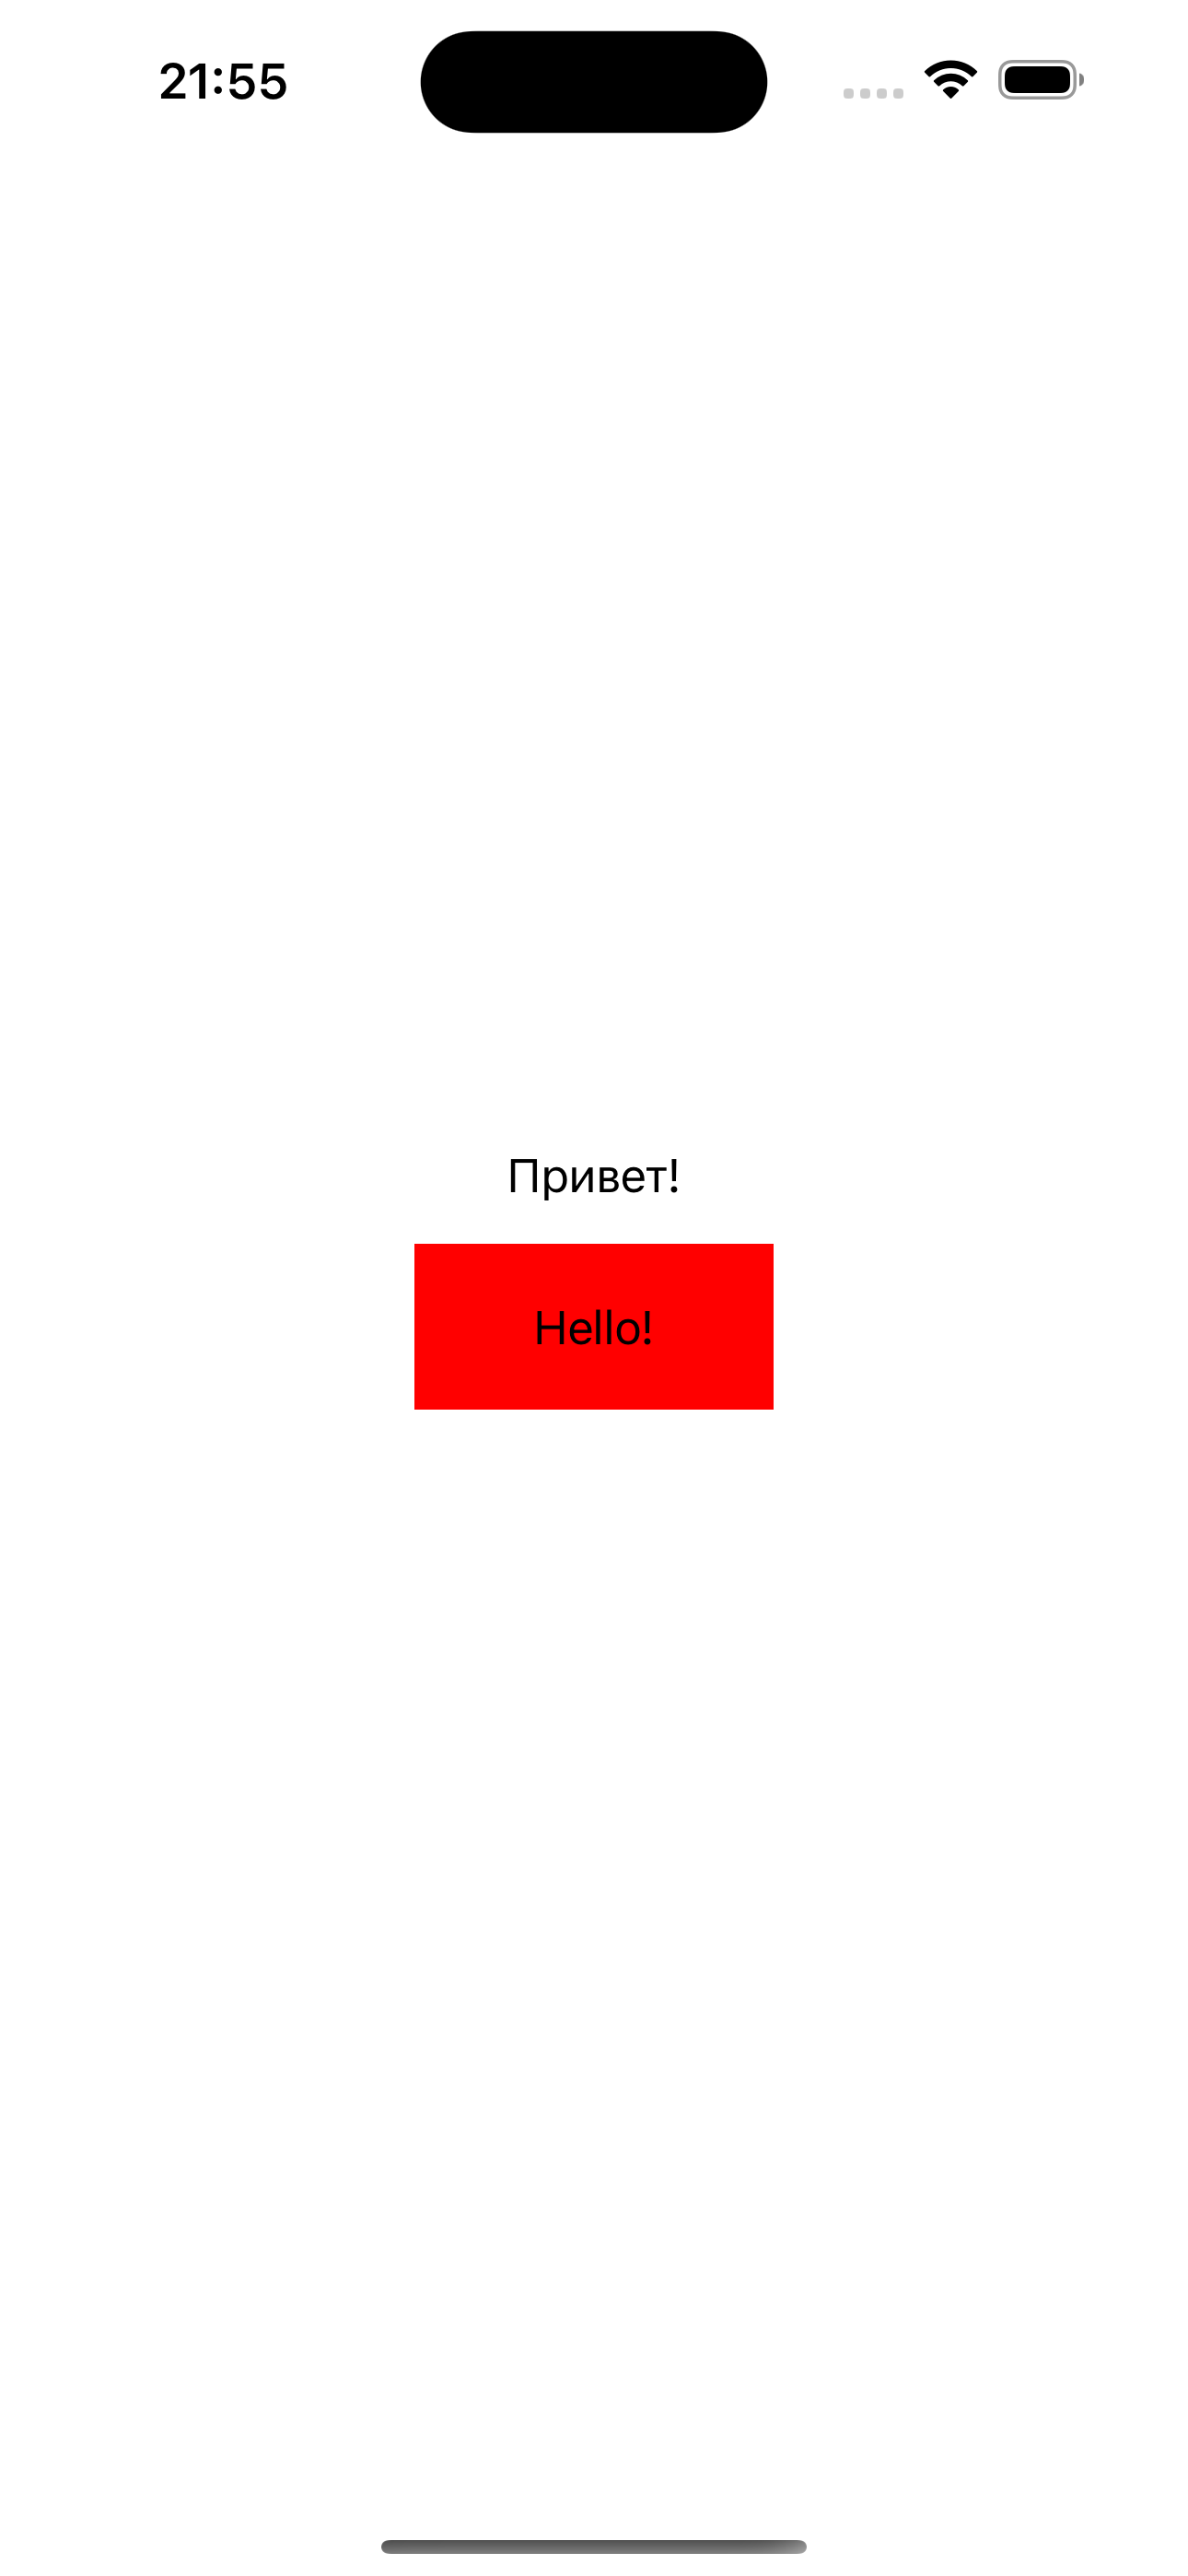
\includegraphics[scale=0.13]{img/example-after.png}
	\caption{Интерфейс после внесения изменений}
	\label{fig:example-after}
\end{figure}
\clearpage
В листинге \ref{code:example-after.xml} представлена разметка XML--файла после внесения изменений.
\begin{code}
	\captionof{listing}{Разметка XML--файла после внесения изменений}
	\label{code:example-after.xml}
	\inputminted
	[
	frame=single,
	framerule=0.5pt,
	framesep=10pt,
	fontsize=\small,
	tabsize=4,
	linenos,
	numbersep=5pt,
	xleftmargin=10pt,
	]
	{text}
	{code/example-after.xml}
\end{code}
\clearpage

\subsubsection{Тестирование}
Разработанное программное обеспечение должно гарантировать корректное отображение задаваемых UI--элементов.
Для этого было проведено snapshot--тестирование, в рамках которого эталонные скриншоты экрана сравниваются с актуальным скриншотами, которые получаются во время прогона тестов.
В качестве эталонных скриншотов используются представления, сверстанные с помощью фреймворка UIKit.
Для выполнения тестирования была использована библиотека SnapshotTesting, предоставляющая весь необходимый для создания snapshot--тестов функционал.

В таблицах 3~---~6 Приложения Б представлен набор тестов, а также результат их выполнения.
Каждый тест предполагает наличие фонового UIView белого цвета.

\subsection*{Вывод}

В данном разделе был обоснован выбор средств программной реализации предлагаемого метода, описан формат входных и выходных данных. 
Разработано программное обеспечение, реализующее представленный метод, приведен пример работы программы, выполнено тестирование, а также описан способ обращения к программе.

\pagebreak